% FIXME Ao final, deixe descomentada a linha correspondente ao numero de paginas
% que a sua defesa possue.
\documentclass[12pt, letterpaper, oneside]{book}  % Para menos de 100 paginas.
% \documentclass[12pt, letterpaper, twoside]{book}  % Para mais de 100 paginas.

%%%%%%%%%%%%%%%%%%%%%%%%%%%% Configuracao: pessoais %%%%%%%%%%%%%%%%%%%%%%%%%%%% 
% FIXME Substituir 'Nome completo do aluno' pelo seu nome.
\newcommand{\autor}{Nome completo do aluno}
% FIXME Se for do sexo feminino, decomente a linha a seguir.
% \def\femaleAuthor{}

% FIXME Substituir 'Titulo da defesa' pelo t�tulo da defesa.
\newcommand{\titulo}{T\'{i}tulo da defesa}
% FIXME Se estiver no programa de mestrado, descomente a linha a seguir.
% \def\mestrado{}
% FIXME Deixe descomente apenas a linha referente ao departamento.
% \def\matematica{}
\def\aplicada{}
% \def\estatistica{}

% FIXME Substituir 'Nome completo do orientador' pelo nome completo do seu
% orientador.
\newcommand{\orientador}{Nome completo do orientador}
% FIXME Se for orientado por uma mulher, descomente a linha a seguir.
% \def\femaleOrientador{}

% FIXME Substituir 'Nome completo do coorientador' pelo nome completo do seu
% coorientador. Caso n�o tenha coorientador, comente a linha a seguir.
\newcommand{\coorientador}{Nome completo do coorientador}
% FIXME Se for coorientado por uma mulher, descomente a linha a seguir.
% \def\femaleCoorientador{}

% FIXME Substituir 'Ano' pelo ano em que ocorreu sua defesa.
\newcommand{\ano}{Ano}

%%%%%%%%%%%%%%%%%%%%%%%%% Configuracao: comportamento %%%%%%%%%%%%%%%%%%%%%%%%%
%%%%%%%%%%%%%%%%%%%%%%%%%%%%%% Pacotes: básicos %%%%%%%%%%%%%%%%%%%%%%%%%%%%%% 
\usepackage[utf8]{inputenc}
\usepackage{cmap}
\usepackage[T1]{fontenc}
\usepackage[brazilian]{babel}
\usepackage{indentfirst}
\usepackage[top=3cm,bottom=3cm,right=2cm,left=2cm]{geometry}


%%%%%%%%%%%%%%%%%%%%%%%%%%%%%%% Pacotes: links %%%%%%%%%%%%%%%%%%%%%%%%%%%%%%%
\usepackage{url}
\usepackage{breakurl}
\usepackage{hyperref}
% FIXME Comente o pacote abaixo quando for concluir sua defesa e for entregar a
% versão final.
\usepackage{showkeys}


%%%%%%%%%%%%%%%%%%%%%%%%%%%%%%%% Pacotes: ams %%%%%%%%%%%%%%%%%%%%%%%%%%%%%%%% 
\usepackage{amsmath}
\usepackage{amsfonts}
\usepackage{amssymb}
\usepackage{amsthm}
\usepackage{breqn}


%%%%%%%%%%%%%%%%%%%%%%%%%%%%%% Pacotes: tabelas %%%%%%%%%%%%%%%%%%%%%%%%%%%%%%
\usepackage{multicol}
\usepackage{multirow}
\usepackage{array}
\usepackage{booktabs}


%%%%%%%%%%%%%%%%%%%%%%%%%%%%%% Pacotes: figuras %%%%%%%%%%%%%%%%%%%%%%%%%%%%%% 
\usepackage{pdfpages}
\usepackage{graphicx}
\usepackage{tikz}
\usepackage{wrapfig}


%%%%%%%%%%%%%%%%%%%%%%%%%%%%% Pacotes: algoritmos %%%%%%%%%%%%%%%%%%%%%%%%%%%%% 
\usepackage{algorithmic}
\usepackage[chapter]{algorithm}
\floatname{algorithm}{Algoritmo}
\renewcommand{\listalgorithmname}{Lista de Algoritmos}


%%%%%%%%%%%%%%%%%%%%%%%%%%%%%% Pacotes: códigos %%%%%%%%%%%%%%%%%%%%%%%%%%%%%% 
\usepackage{textcomp}
\usepackage{listings}
\renewcommand\lstlistingname{Código}
\renewcommand\lstlistlistingname{Lista de Códigos}


%%%%%%%%%%%%%%%%%%%%%%%%%%%%%%% Pacotes: index %%%%%%%%%%%%%%%%%%%%%%%%%%%%%%% 
\usepackage{makeidx}
\makeindex


%%%%%%%%%%%%%%%%%%%%%%%%%%%%%%% Pacotes: fontes %%%%%%%%%%%%%%%%%%%%%%%%%%%%%% 
\usepackage{lmodern}
\usepackage{mathrsfs}


% TODO Inserir pacotes adicionais aqui.
  % Arquivo com os pacotes.
%%%%%%%%%%%%%%%%%%%%%%%%%% Configuração: frontmatter %%%%%%%%%%%%%%%%%%%%%%%%%%
\appto\frontmatter{\pagestyle{plain}}  % Adiciona o estilo plano de página.


%%%%%%%%%%%%%%%%%%%%%%%%%% Configurações: referências %%%%%%%%%%%%%%%%%%%%%%%%%%
\addbibresource{tese.bib}


%%%%%%%%%%%%%%%%%%%%%%%%%%%%% Configurações: links %%%%%%%%%%%%%%%%%%%%%%%%%%%%%
\hypersetup{
% TODO Por padrão os links, no pdf, para equações, figuras, referencias,
% tabelas, urls são identificados por uma caixa colorida em volta do link. Essa
% caixa colorida não eh impressa mas pode atrapalhar a leitura para alguns. Se
% desejar removê-las descomente a linha abaixo.
% hidelinks,
hypertexnames=false,
pdftitle={\titulo},  % Não modifique esta linha.
pdfauthor={\autor}  % Não modifique esta linha.
}


%%%%%%%%%%%%%%%%%%%%%%%%%% Configurações: numeração %%%%%%%%%%%%%%%%%%%%%%%%%%
\numberwithin{equation}{section}
\numberwithin{section}{chapter}


%%%%%%%%%%%%%%%%%%%%%%%%%%%%% Configurações: ams %%%%%%%%%%%%%%%%%%%%%%%%%%%%%
\theoremstyle{definition}
\newtheorem{thm}{Teorema}[section]
\newtheorem{con}[thm]{Conjectura}
\newtheorem{cor}[thm]{Corolário}
\newtheorem{dfn}[thm]{Definição}
\newtheorem{exm}[thm]{Exemplo}
\newtheorem{lem}[thm]{Lema}
\newtheorem{obs}[thm]{Observação}
\newtheorem{pps}[thm]{Proposição}


%%%%%%%%%%%%%%%%%%%%%%%%%% Configurações: algoritmos %%%%%%%%%%%%%%%%%%%%%%%%%%
\algsetup{linenosize=\small}
\renewcommand{\algorithmicrequire}{\textbf{Entrada:}}
\renewcommand{\algorithmicensure}{\textbf{Saída:}}
\renewcommand{\algorithmicend}{\textbf{fim}}
\renewcommand{\algorithmicif}{\textbf{se}}
\renewcommand{\algorithmicthen}{\textbf{ent\~{a}o}}
\renewcommand{\algorithmicelse}{\textbf{caso contr\'{a}rio}}
\renewcommand{\algorithmicendif}{\algorithmicend}
\renewcommand{\algorithmicfor}{\textbf{para}}
\renewcommand{\algorithmicforall}{\textbf{para todo}}
\renewcommand{\algorithmicdo}{\textbf{fa\c{c}a}}
\renewcommand{\algorithmicendfor}{\algorithmicend}
\renewcommand{\algorithmicwhile}{\textbf{enquanto}}
\renewcommand{\algorithmicendwhile}{\algorithmicend}
\renewcommand{\algorithmicrepeat}{\textbf{repita}}
\renewcommand{\algorithmicuntil}{\textbf{at\'{e}}}
\renewcommand{\algorithmicreturn}{\textbf{retorne}}
\renewcommand{\algorithmiccomment}[1]{\hspace{2em}/* #1 */}


%%%%%%%%%%%%%%%%%%%%%%%%%%%%%% Configurações: códigos %%%%%%%%%%%%%%%%%%%%%%%% 
\lstset{
basicstyle=\ttfamily,
keywordstyle=\bfseries\color{green!40!black},
commentstyle=\color{gray},
stringstyle=\color{Maroon},
identifierstyle=\color{Blue},
numbers=left,
numberstyle=\tiny,
breaklines=false
}


%%%%%%%%%%%%%%%%%%%%%%%%%%%%% Configurações: anexo %%%%%%%%%%%%%%%%%%%%%%%%%%%
\newcommand{\annexname}{Anexo}
\makeatletter
\newcommand\annex{\par
\setcounter{chapter}{0}%
\setcounter{section}{0}%
\gdef\@chapapp{\annexname}%
\gdef\thechapter{\@Roman\c@chapter}}
\makeatother


% TODO Inserir configurações adicionais aqui.
  % Arquivo com algumas configuracoes.

%%%%%%%%%%%%%%%%%%%%%%%%%% Inicio do texto da defesa %%%%%%%%%%%%%%%%%%%%%%%%%%
\begin{document}
% WARNING Todas as paginas deverao ser numeradas.
%
% As paginas iniciais sao numeradas com algorimos romanos em sua forma
% minuscula.
\frontmatter
%
\thispagestyle{plain}
\includegraphics[width=.94in, height=1in,
keepaspectratio=true]{figuras/unicamp-logo}
\vspace*{.8cm}
\begin{center}
  % O tamanho da fonte deve ser 16pt.
  % Deve-se utilizar caixa alta.
  {\Large\textsc{\autor}}
\end{center}
\vspace{1.9cm}
\begin{center}
  % O tamanho da fonte deve ser 16pt em negrito.
  % Deve-se utilizar caixa alta.
  {\Large\textbf{\textsc{\titulo}}}
\end{center}
\vspace{2.2cm}
\begin{center}
  % O tamanho da fonte deve ser 16pt em negrito.
  % Deve-se utilizar caixa alta.
  {\Large\textsl{\textsc{\titulopt}}}
\end{center}
\vfill
\begin{center}
  % O tamanho da fonte deve ser 12pt em negrito.
  % Deve-se utilizar caixa alta.
  \textbf{CAMPINAS \\ \ano}
\end{center}
  % Nao edite esse arquivo.
\newpage\mbox{}\thispagestyle{plain}\newpage  % Pagina em branco.
%
% WARNING A folha de rosto precisa ser assinada pelos orientadores.
% FIXME Substitua arquivo folha-de-rosto.pdf por uma copia escaneada, comente
% esta linha e descomente a proxima.
\thispagestyle{plain}
% WARNING Não modifique este arquivo.
\includegraphics[width=.94in, height=1in,
keepaspectratio=true]{figuras/unicamp-logo}
\begin{center}
  {\large \scshape \bfseries Universidade Estadual de Campinas
  \vspace{.5cm}

  Instituto de Matemática, Estatística \\
  e Computação Científica}
\end{center}
\vfill
\begin{center}
  {\large \scshape \bfseries \autor}
\end{center}
\vfill
\begin{center}
  {\Large \scshape \bfseries \titulo}
\end{center}
\vfill

\begin{flushright}
  \begin{minipage}[c]{.5\textwidth}
    \ifx\mestrado\undefined
    Tese
    \else
    Dissertação
    \fi
    apresentada ao Instituto de Matemática,
    Estatística e Computação Científica da Universidade
    Estadual de Campinas como parte dos requisitos exigidos
    para a obtenção do título de
    \ifx\mestrado\undefined
    \ifx\femaleAuthor\undefined
    Doutor
    \else
    Doutora
    \fi
    \else
    \ifx\femaleAuthor\undefined
    Mestre
    \else
    Mestra
    \fi
    \fi
    em
    \ifx\matematica\undefined
    \else
    matemática.
    \fi
    \ifx\aplicada\undefined
    \else
    matemática aplicada.
    \fi
    \ifx\estatistica\undefined
    \else
    estatística.
    \fi
  \end{minipage}
\end{flushright}
\vspace{.5cm}

\noindent
{\bfseries
\noindent
Orientador\ifx\femaleOrientador\undefined
\else
a\fi: \orientador
\vspace{.25cm}

\ifx\coorientador\undefined
\else
\noindent
Coorientador\ifx\femaleCoorientador\undefined
\else
a\fi: \coorientador
\fi
}
\vspace{.5cm}

\noindent
\begin{minipage}[c]{.5\textwidth}
  \noindent
  {\footnotesize \scshape
  Este exemplar corresponde à versão final da
  \ifx\mestrado\undefined
  tese
  \else
  dissertação
  \fi
  defendida
  \ifx\femaleAuthor\undefined
  pelo aluno
  \else
  pela aluna
  \fi
  \autor,
  e orientada pel\ifx\femaleOrientador\undefined
  o\else
  a\fi{} Prof\ifx\femaleOrientador\undefined
  \else
  a\fi. Dr\ifx\femaleOrientador\undefined
  \else
  a\fi. \orientador.
  }
\end{minipage}
\vspace{1cm}

\noindent
{\small \bfseries
\noindent
Assinatura
\ifx\femaleOrientador\undefined
do Orientador
\else
da Orientadora
\fi

\vspace{.5cm}
\noindent
\rule[1pt]{7cm}{.5pt}  % Linha para assinatura do orientador
}
\vspace{.5cm}


\ifx\coorientador\undefined
\else
{\small \bfseries
\noindent
Assinatura
\ifx\femaleCoorientador\undefined
do Coorientador
\else
da Coorientadora
\fi

\vspace{.5cm}
\noindent
\rule[1pt]{7cm}{.5pt}  % Linha para assinatura do coorientador
}
\fi
\vfill
\begin{center}
  {\small \scshape \bfseries Campinas \\ \ano}
\end{center}

% \includepdf{folha-de-rosto.pdf}
%
% WARNING A ficha catalografica deve estar no verso da folha de rosto.
% FIXME O arquivo ficha-catalografica.pdf deve ser sobrescrito com uma c�pia
% do arquivo pdf que a bibliotaca lhe enviar.
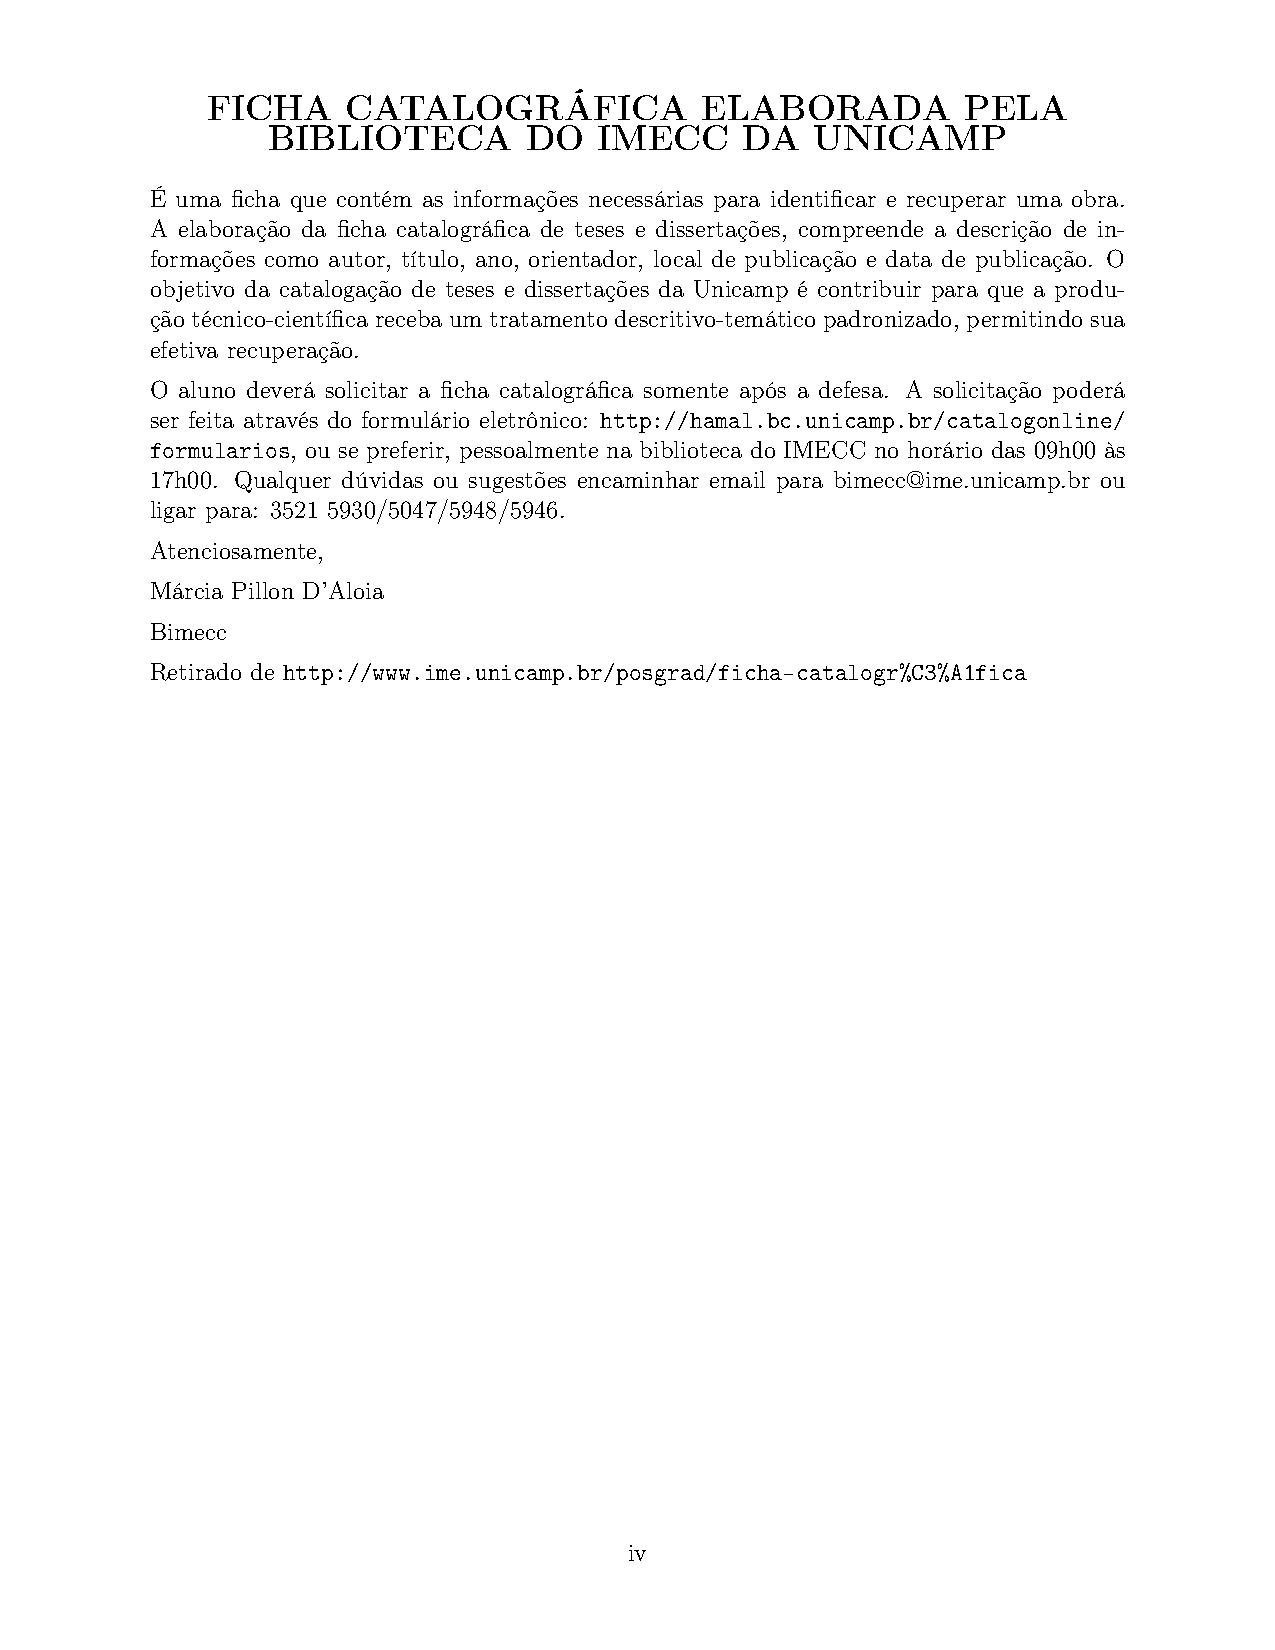
\includepdf{ficha-catalografica}
%
% WARNING A folha de aprovacao deve ser assinada pelos membros da banca apos a
% defesa.
% FIXME Substitua o arquivo folha-de-aprovacao.pdf por uma copia escaneada.
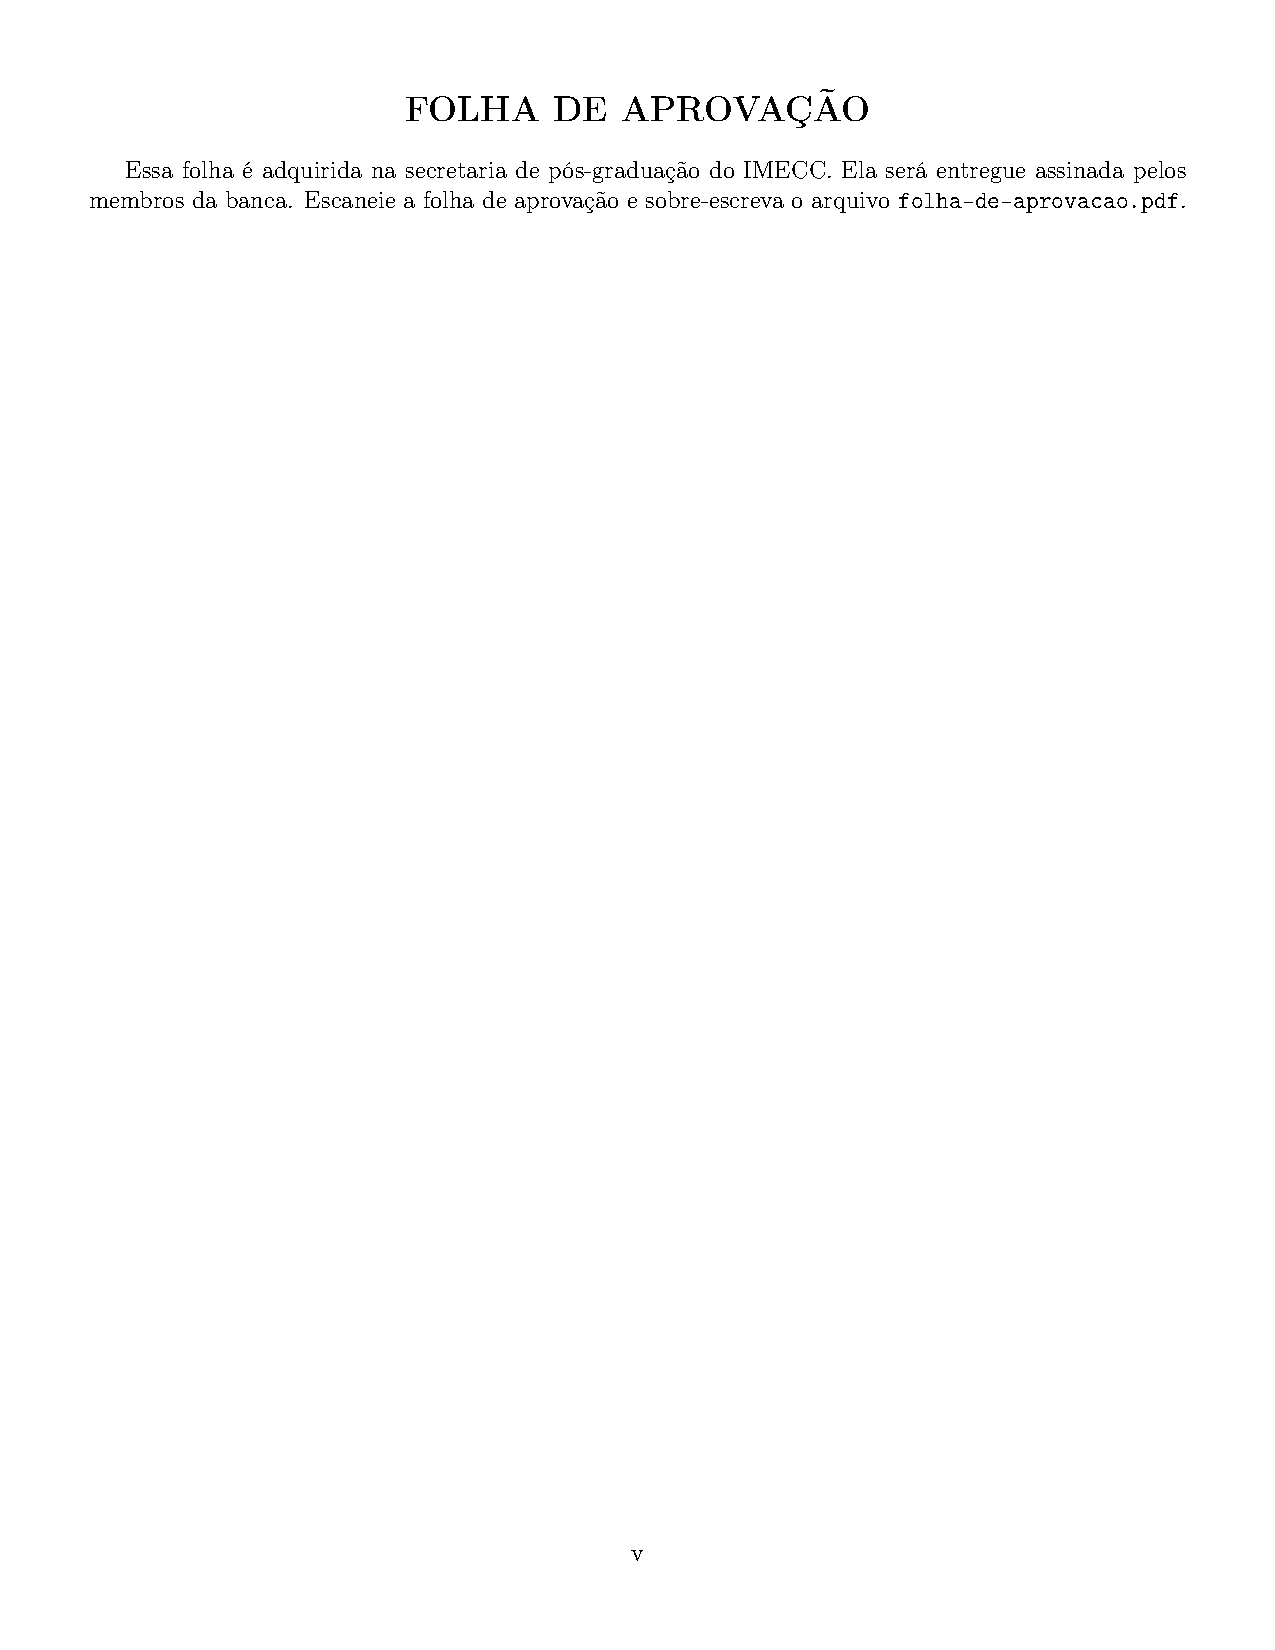
\includepdf{folha-de-aprovacao}
%
% FIXME Se n�o for incluir a dedicat�ria, comentar a linha abaixo.
\chapter*{}
\begin{center}
    \emph{
    % FIXME Remover as duas linhas abaixo.
    Aos meus \ldots. \\
    Para \ldots.} 
    % TODO Inserir a dedicatória aqui.
\end{center}

%
% FIXME Se n�o for incluir a epigrafe, comentar a linha abaixo.
%%TODO Escrever o modelo da epigrafe.
\chapter*{}
\vfill
\begin{flushright}
  Epígrafe \\
  Epígrafe \\
  Epígrafe \\
  Epígrafe
\end{flushright}

%
% FIXME Se n�o for incluir os agradecimentos, comentar a linha abaixo.
\chapter*{Agradecimentos}
% FIXME Escrever os agradecimentos.
Aqui deve-se agradecer quem merece agradecimento

Se recebeu bolsa de algum órgão de fomento, não esqueça de agradecê-lo.

%
\begin{center}
    {\bf Resumo}
\end{center}
\addcontentsline{toc}{chapter}{Resumo}

% FIXME Remover as 3 linhas abaixo.
resumo resumo resumo
resumo resumo resumo
resumo resumo resumo
% TODO Inserir o resume em portugês aqui.

\vspace{2cm}
\textbf{Palavras-chave}:
% FIXME Remover a linha abaixo.
palavra01, palavra02, palavra03.
% TODO Inserir as palavras-chave aqui.

\clearpage
\begin{center}
    {\bf Abstract}
\end{center}
\addcontentsline{toc}{chapter}{Abstract}

% FIXME Remover as 3 linhas abaixo.
abstract abstract abstract
abstract abstract abstract
abstract abstract abstract
% TODO Inserir o resume em inglês aqui.

\vspace{2cm}
\textbf{Keywords}:
% FIXME Remover a linha abaixo.
keyword01, keyword02, keyword03.
% TODO Inserir as palavras-chave em inglês aqui.

%
\tableofcontents
% FIXME Comentar as linhas abaixo de n�o desejar listar as figuras
% apresentadas.
\listoffigures
\addcontentsline{toc}{chapter}{Lista de Figuras}
%
% FIXME Comentar as linhas abaixo de n�o desejar listar as tabelas
% apresentadas.
\listoftables
\addcontentsline{toc}{chapter}{Lista de Tabelas}
%
% FIXME Comentar as linhas abaixo de n�o desejar listar os
% algoritmos apresentados.
\listofalgorithms
\addcontentsline{toc}{chapter}{Lista de Algoritmos}
%
% FIXME Comentar as linhas abaixo de n�o desejar listar os trechos de c�digo
% apresentados.
\lstlistoflistings
\addcontentsline{toc}{chapter}{Lista de C\'{o}digos}
%
% FIXME Comentar a linha abaixo de n�o for apresentar as
% abrevia��es utilizadas.
\noindent{\Huge\bf Abrevia\c{c}\~{o}es}
\addcontentsline{toc}{chapter}{Abrevia\c{c}\~{o}es}

\begin{description}
    % FIXME Remover as duas abrevia\c{c}\~{o}es abaixo e incluir as que ser\~{a}o
    % utilizadas.
    \item[FIXME] Indica que algo deve ser consertado.
    \item[TODO] Indica que algo deve ser feito.
\end{description}

%
% FIXME Comentar a linha abaixo de n�o for apresentar os
% s�mbolos utilizados.
\chapter*{Símbolos}

\begin{description}
    % FIXME Remover os dois símbolos abaixo e incluir as que serão
    % utilizadas.
    \item[$\diamond$] Representa um diamante.
    \item[$\lhd$] Representa um deslocamento para a esquerda.
    \item[$\rhd$] Representa um deslocamento para a direita.
\end{description}

%
% FIXME Comentar a linha abaixo de n�o for apresentar o
% glossario.
\chapter{Gloss\'{a}rio}
\addcontentsline{toc}{chapter}{Glossário}

%%TODO Escrever o exemplo de glossario.

%
% As paginas com o conteudo da tese sao numeradas com algorimos arabicos.
\mainmatter
%
% FIXME Remover as 3 linhas abaixo.
\chapter{Título 1}
Esse é o primeiro capítulo da sua tese.

\section{Seção 1.1}
Essa é uma seção da sua tese.

\subsection{Subseção 1.1.1}

Essa é uma subseção da sua tese.

\subsection{Subseção 1.1.2}

Essa é outra subseção da sua tese.

\section{Equações matemáticas}
Para equações matemáticas está sendo utilizado os seguintes
pacotes:
\begin{itemize}
  \item amsmath,
  \item amsfonts,
  \item amssymb,
  \item amsthm,
  \item breqn.
\end{itemize}

Um exemplo de equação na mesma linha: 
$ 1 + 1 + 1 + 1 + 1 + 1 = 6$, 
que é trivial\index{trivial} de ser verificada.

Equações na mesma linha são quebradas automaticamente:
$ 1 + 1 + 1 + 1 + 1 + 1 + 1 + 1 + 1 + 1 + 1 + 1 = 12$. 

Ao utilizar equações na mesma linha deve-se tomar o cuidado de manter a
legibilidade da equação e não modificar a altura da linha. É
errado utilizar $\frac{1}{2} + \frac{1}{2} = 1$ ou $\frac{\partial}{\partial x}
(y^2 + 2xy + x^2) = 2y + 2x$, devendo ser utilizado $(1/2) + (1/2) = 1$ ou
$\partial (y^2 + 2 x y + x^2) / \partial x = 2 y + 2 x$.

Além de equações na mesma linha, também é possível
utilizar equações em destaque:
\begin{equation}
  1 + 1 + 1 + 1 + 1 + 1 = 6
\end{equation}
ou
\begin{equation*}
  1 + 1 + 1 + 1 + 1 + 1 = 6.
\end{equation*}
Ao utilizar equações matemáticas em destaque, não esqueça da pontuação nas
equações.

Recomenda-se utilizar os ambientes
\begin{itemize}
  \item dmath(*) e
  \item dgroup(*)
\end{itemize}
disponibilizados pelo pacote breqn ao invés dos ambientes
\begin{itemize}
  \item equation(*,)
  \item align(*),
  \item multiline(*) e
  \item split
\end{itemize}
pois os primeiros quebram e alinham automaticamente as equações em destaque.
Veja a seguir a ``equivalência'' entre os ambientes:
\begin{description}
  \item[dmath]
    \begin{dmath}
      1 + 1 + 1 + 1 + 1 + 1 + 1 + 1 + 1 + 1 + 1 + 1 + 1 + 1 + 1 + 1 + 1 + 1 + 1
      + 1 + 1 + 1 + 1 + 1 + 1 + 1 + 1 + 1 + 1 + 1 = 30
    \end{dmath}
  \item[equation] 
    \begin{equation}
      1 + 1 + 1 + 1 + 1 + 1 + 1 + 1 + 1 + 1 + 1 + 1 + 1 + 1 + 1 + 1 + 1 + 1 + 1
      + 1 + 1 + 1 + 1 + 1 + 1 + 1 + 1 + 1 + 1 + 1 = 30
    \end{equation}
  \item[equation com split] 
    \begin{equation}
      \begin{split}
        1 + 1 + 1 + 1 + 1 + 1 + 1 + 1 + 1 + 1 + 1 + 1 + 1 + 1 + 1 \\
        + 1 + 1 + 1 + 1 + 1 + 1 + 1 + 1 + 1 + 1 + 1 + 1 + 1 + 1 + 1 = 30 
      \end{split}
    \end{equation}
  \item[align] 
    \begin{align}
      1 + 1 + 1 + 1 + 1 + 1 + 1 + 1 + 1 + 1 + 1 + 1 + 1 + 1 + 1 \\
      + 1 + 1 + 1 + 1 + 1 + 1 + 1 + 1 + 1 + 1 + 1 + 1 + 1 + 1 + 1 = 30 
    \end{align}
  \item[align com quebra de linha] 
    \begin{align}
      1 + 1 + 1 + 1 + 1 + 1 + 1 + 1 + 1 + 1 + 1 + 1 + 1 + 1 + 1 \\
      + 1 + 1 + 1 + 1 + 1 + 1 + 1 + 1 + 1 + 1 + 1 + 1 + 1 + 1 + 1 = 30 
    \end{align}
\end{description}

No caso do desenvolvimento/simplificação de uma expressão
matemática também é recomendado utilizar os ambientes
disponibilizados pelo pacote breqn.
\begin{description}
  \item[dmath]
    \begin{dmath}
      f(x) = 1 + 1 + 1 + 1 + 1 + 1 + 1 + 1 + 1 + 1 + 1 + 1 + 1 + 1 + 1 + 1 + 1 +
      1 + 1 + 1 + 1 + 1 + 1 + 1 + 1 + 1 + 1 + 1 + 1 + 1
      = 2 + 2 + 2 + 2 + 2 + 2 + 2 + 2 + 2 + 2 + 2 + 2 + 2 + 2 + 2
      = 4 + 4 + 4 + 4 + 4 + 4 + 4 + 2
      = 8 + 8 + 8 + 6
      = 16 + 14
      = 30
    \end{dmath}
  \item[equation com split] 
    \begin{equation}
      \begin{split}
        f(x) &= 1 + 1 + 1 + 1 + 1 + 1 + 1 + 1 + 1 + 1 + 1 + 1 + 1 + 1 + 1 + 1 + 1 \\
        &\quad {}+ 1 + 1 + 1 + 1 + 1 + 1 + 1 + 1 + 1 + 1 + 1 + 1 + 1 \\
        &= 2 + 2 + 2 + 2 + 2 + 2 + 2 + 2 + 2 + 2 + 2 + 2 + 2 + 2 + 2 \\
        &= 4 + 4 + 4 + 4 + 4 + 4 + 4 + 2 \\
        &= 8 + 8 + 8 + 6 \\
        &= 16 + 14 \\
        &= 30
      \end{split}
    \end{equation}
  \item[align com quebra de linha] 
    \begin{align}
        f(x) &= 1 + 1 + 1 + 1 + 1 + 1 + 1 + 1 + 1 + 1 + 1 + 1 + 1 + 1 + 1 + 1 + 1 \\
        &\quad {}+ 1 + 1 + 1 + 1 + 1 + 1 + 1 + 1 + 1 + 1 + 1 + 1 + 1 \\
        &= 2 + 2 + 2 + 2 + 2 + 2 + 2 + 2 + 2 + 2 + 2 + 2 + 2 + 2 + 2 \\
        &= 4 + 4 + 4 + 4 + 4 + 4 + 4 + 2 \\
        &= 8 + 8 + 8 + 6 \\
        &= 16 + 14 \\
        &= 30
    \end{align}
\end{description}

Para o caso de equações relacionadas e que devem ser agrupadas,
temos
\begin{description}
  \item[dgroup com dmath]
    \begin{dgroup}
      \begin{dmath}
        f(x) = 1 + 1 + 1 + 1 + 1 + 1 + 1 + 1 + 1 + 1 + 1 + 1 + 1 + 1 + 1 + 1 + 1
        + 1 + 1 + 1 + 1 + 1 + 1 + 1 + 1 + 1 + 1 + 1 + 1 + 1
        = 2 + 2 + 2 + 2 + 2 + 2 + 2 + 2 + 2 + 2 + 2 + 2 + 2 + 2 + 2
        = 4 + 4 + 4 + 4 + 4 + 4 + 4 + 2
        = 8 + 8 + 8 + 6
        = 16 + 14
        = 30
      \end{dmath}
      \begin{dmath}
        g(x) = 2 + 2 + 2 + 2
        = 4 + 4
        = 8
      \end{dmath}
    \end{dgroup}
  \item[subequations com equation com split] 
    \begin{subequations}
      \begin{equation}
        \begin{split}
          f(x) &= 1 + 1 + 1 + 1 + 1 + 1 + 1 + 1 + 1 + 1 + 1 + 1 + 1 + 1 + 1 + 1 + 1 \\
          &\quad {}+ 1 + 1 + 1 + 1 + 1 + 1 + 1 + 1 + 1 + 1 + 1 + 1 + 1 \\
          &= 2 + 2 + 2 + 2 + 2 + 2 + 2 + 2 + 2 + 2 + 2 + 2 + 2 + 2 + 2 \\
          &= 4 + 4 + 4 + 4 + 4 + 4 + 4 + 2 \\
          &= 8 + 8 + 8 + 6 \\
          &= 16 + 14 \\
          &= 30
        \end{split}
      \end{equation}
      \begin{equation}
        \begin{split}
          g(x) &= 2 + 2 + 2 + 2 \\
          &= 4 + 4 \\
          &= 8
        \end{split}
      \end{equation}
    \end{subequations}
  \item[align com split] 
    \begin{align}
      \begin{split}
        f(x) &= 1 + 1 + 1 + 1 + 1 + 1 + 1 + 1 + 1 + 1 + 1 + 1 + 1 + 1 + 1 + 1 + 1 \\
        &\quad {}+ 1 + 1 + 1 + 1 + 1 + 1 + 1 + 1 + 1 + 1 + 1 + 1 + 1 \\
        &= 2 + 2 + 2 + 2 + 2 + 2 + 2 + 2 + 2 + 2 + 2 + 2 + 2 + 2 + 2 \\
        &= 4 + 4 + 4 + 4 + 4 + 4 + 4 + 2 \\
        &= 8 + 8 + 8 + 6 \\
        &= 16 + 14 \\
        &= 30
      \end{split} \\
      \begin{split}
        g(x) &= 2 + 2 + 2 + 2 \\
        &= 4 + 4 \\
        &= 8
      \end{split}
    \end{align}
\end{description}

\subsection{Referência cruzada}
Parte das equações anteriores encontram-se numeradas. Esse número pode ser
facilmente acessado se junto da equação tiver sido utilizando o comando label:
\begin{dmath}
  c^2 = a^2 + b^2. \label{eq:exem_pitagoras}
\end{dmath}
E para acessar o número utiliza o comando eqref, \eqref{eq:exem_pitagoras}.

Além de numerar equações também é possível nomeá-las utilizando o comando
tag\footnote{O pacote breqn não possue suporte ao comando tag.}:
\begin{align}
  c^2 &= a^2 + b^2 - 2 a b \cos\theta 
  \label{eq:exem_pitagoras_generalizado}
  \tag{GTP}
\end{align}
E para acessar o nome utiliza-se o comando eqref,
\eqref{eq:exem_pitagoras_generalizado}.

Para que no pdf não apareça o parâmetro dos comandos label é preciso remover o
pacote showlabels do arquivo pacotes.tex.

\section{Definições}
Vários ambientes já estão definidos como: Teorema, Conjectura, Corolário,
Definição, \ldots

\begin{thm}
  Teorema, Teorema, Teorema, Teorema.
\end{thm}

\begin{con}
  Conjectura, Conjecture, Conjectura, Conjectura.
\end{con}

\begin{cor}
  Corolário, Corolário, Corolário, Corolário.
\end{cor}

\begin{dfn}
  Definição, Definição, Definição.
\end{dfn}

Use esses ambientes de maneira sábia.

\chapter{Título 2}
Esse é o segundo capítulo da sua defesa.

\section{Seção 2.1}
Essa é uma seção da sua defesa.

É possível inserir figuras na sua defesa. \\

\includegraphics{figuras/unicamp-logo.jpg}

É recomendado deixar as figuras\index{figura} como objetos flutuantes.
\begin{figure}[!htb]
  \center
  
\includegraphics[width=4cm]{figuras/unicamp-logo.jpg}
  \caption{Logo da UNICAMP.}
  \label{fig:log_unicamp}
\end{figure}

Além de inserir figuras é possível ``desenhar''\index{figura!desenhar} figuras
utilizando o pacote TikZ\index{figura!TikZ}, como na Figura~\ref{fig:exem_tikz}.
\begin{figure}[!htb]
  \centering
  \begin{tikzpicture}
    \draw (0,0) -- (0,2) -- (2,2) -- (2,0) -- (0,0);
  \end{tikzpicture}
  \caption{Exemplo do uso do TikZ.}
  \label{fig:exem_tikz}
\end{figure}

\section{Seção 2.2}
Além de figuras também é possível inserir tabelas. \\
\begin{tabular}{cc}
  \toprule
  Tabela & Tabela \\
  \midrule
  Tabela & Tabela \\
  \bottomrule
\end{tabular}

Assim como as figuras, é recomendado que as tabelas sejam incluídas como
objetos flutuantes.
\begin{table}[!htb]
  \caption{Exemplo de Tabela.}
  \label{tab:exem}
  \centering
  \begin{tabular}{cc}
    \toprule
    Tabela & Tabela \\
    \midrule
    Tabela & Tabela \\
    \bottomrule
  \end{tabular}
\end{table}

Além de inserir tabelas manualmente, como na Tabela~\ref{tab:exem}, também é
possível utilizar arquivos \emph{.csv} para criar tabelas. Neste caso, é
necessário incluir o pacote \texttt{csvsimple} que não foi incluído por questão
de compatibilidade com distribuições do \LaTeX \ anteriores a 2009.

\chapter{T\'itulo 3}
Esse \'e o terceiro cap\'itulo da sua tese.

\section{Se\c c\~ao 3.1}
Para facilitar a leitura, é bom incluir o algoritmo de forma adequada e não
como uma lista.
\begin{algorithmic}[2]
    \STATE $i \leftarrow 0$
    \STATE $y \leftarrow 0$
    \FOR{$i \leq 10$}
        \STATE $y \leftarrow y + i$
        \STATE $i \leftarrow i + 1$
    \ENDFOR
\end{algorithmic}

É possível nomear os algoritmos\index{algoritmo}.
\begin{algorithm}
    \caption{Loop infinito.}
    \label{alg:loop_inf}
    \begin{algorithmic}
        \REQUIRE $n \geq 0$
        \ENSURE $y = 1 + 2 + \ldots + n$
        \STATE $y \leftarrow 0$
        \STATE $i \leftarrow 0$
        \IF{$n < 0$}
            \PRINT Entrada inadequada.
        \ELSE
            \WHILE{$i \neq n$}
                \STATE $y \leftarrow y + i$
            \ENDWHILE
        \ENDIF
    \end{algorithmic}
\end{algorithm}

Para algoritmos, recomenda-se utilizar o pacote
\emph{algorithmic}\index{algoritmo!algorithmic@\emph{algorithmic}} pois este
permite a tradução dos ``comandos''.

Em alguns casos, recomenda-se incluir um trecho de
código\index{codigo@c\'{o}digo}.
\lstinputlisting[firstline=5, lastline=5, nolol=true]{src/exem.c}

Assim como os algoritmos também é possível nomear os códigos.
\lstinputlisting[firstline=10, lastline=12, caption=Loop em C,
language=C,  frame=single]{src/exem.c}

Para trecho de códigos,  recomenda-se utilizar o pacote
\emph{listings}\index{codigo@c\'{o}digo!listings@\emph{listings}} pois
este possue várias opções.

% TODO Inserir os arquivos referentes ao corpo da tese.
%
% FIXME Se nao for utilizar apendices ou anexos, comentar a linha abaixo.
\appendix
% FIXME Remover as 2 linhas abaixo.
\chapter{Título A}
Esse é um Apêndice da sua tese.

\section{Seção A.1}
Essa é uma seção de um dos apêndices da sua tese.

\chapter*{Anexo}
\addcontentsline{toc}{chapter}{Anexo}
Esse é um anexo.

% TODO Inserir os arquivos referentes aos apendices e anexos.
%
\backmatter
% FIXME Remover a linha abaixo.
\nocite{*}
% FIXME Mudar o estilo para o de sua preferencia.
\bibliographystyle{amsplain}
% FIXME Adicionar os arquivos .bib que for utilizar ou editar o arquivo
% tese.bib.
\bibliography{tese}
\addcontentsline{toc}{chapter}{Refer\^{e}ncia Bibliogr\'{a}fica}
%
\clearpage
\addcontentsline{toc}{chapter}{\'{I}ndice Remissivo}
\printindex
\end{document}
